\chapter*{Wizard Tower of Dundee}\stepcounter{chapter}\phantomsection\addcontentsline{toc}{chapter}{Wizard Tower of Dundee}
\noindent \textit{Feel free to treat this puzzle-filled Wizard Tower as an optional side-quest. It exists simply to give your group a light, puzzle-focused break before the \hyperref[chapter:UnicornInvasionOfDundee]{\LinkFont{Unicorn Invasion of Dundee}} truly unfolds. Since the invasion deserves its own dedicated session (and shouldn't be broken up), this adventure lets you occupy a play session with clever challenges and exploration before diving headlong into the spectacular battle to come.}\\
\DndDropCapLine{U}{\entryfont pon arriving at the Wizard Tower of Dundee, the party encounters a magnificent wooden door set into the stone façade. Its surface is covered in intricate, fading runes and arcane depictions - stars, planetary symbols, and scenes of spellcasting - yet years of neglect have left it streaked with rusted metal fittings and patches of moss clinging to its edges.}

\begin{DndReadAloud}
	As you step onto the cobblestones of Dundee's wizard quarter, the Tower of Dundee looms above you - a spiraling gray stone keep etched with glowing runes. Set into the base of its wall is a grand wooden door, once opulent, now aged and weathered. Intricate arcane symbols and depictions of spellcasters cover its panels, but rusted iron straps streak across the wood, and patches of moss curl around its edges, as if nature itself seeks to reclaim it.

	Before you can examine it further, a young woman in immaculate azure robes approaches, her robes embroidered with the tower's crest. Her lips curve into a polite but condescending smile as she crosses her arms.

	\textit{"And what, may I ask"}, she says in a crisp, clipped tone, \textit{"draws you to the Tower of Dundee? Curiosity, ambition, or something else entirely?"}
\end{DndReadAloud}

{\noindent\entryfont No matter how the door is opened - lockpicking, kicking it in, or casting Knock - the moment the door yields by any means (or the word "Time" is spoken nearby), a hidden ward activates. Instantly, every member of the party and the snooty student Eilidh MacKenzie are thrown into separate puzzle chambers within the tower.}

\section*{Puzzle Rooms}\phantomsection\addcontentsline{toc}{section}{Puzzle Rooms}
{\entryfont This segment presents a sample framework for the puzzle chambers that lie beyond the warded door. Feel free to design entirely new challenges tailored to your group - this example is merely illustrative. In it, each player is whisked into a distinct room shaped by their character's (sub-)class, while a central chamber remains pitch black. Eilidh MacKenzie, who always lands in the darkened hub, knows the Light Cantrip and will harshly scold any spellcaster there who can't cast it.}

\subsection*{Central Chamber}
\textbf{{\entryfont Correct Combination:} 947}\\
{\entryfont The central chamber is magically linked to all outer rooms, allowing occupants of those rooms to communicate with the central hub, but the outer rooms cannot do so directly with one another.}

\begin{DndReadAloud}
	As the ward's magic ripples through you, darkness swallows your senses. You feel the chill of damp stone beneath your feet and hear distant, echoing drops of water. Soon after, a single point of light ignites near your shoulder - Eilidh glares at you from across the void, her fingertips aflame with a soft, bluish glow.
	
	Around you, three round stone pillars loom out of the black: each carved with ten faintly recessed glyphs depicting the digits 0 through 9 in a clockwise ring. In front of the middle stele stands a tall, conical funnel of weathered stone, crowned by a gigantic, multifaceted crystal that seems to pulse with arcane energy. A simple wooden table nearby holds a lone sheet of parchment.
\end{DndReadAloud}

{\noindent\entryfont Within this chamber, the party must piece together a three-digit code by interpreting the riddle on the \hyperref[resource:WizardTowerPuzzleRiddle]{\LinkFont{Parchment}} and find clues in each outer room. Once they believe they have the correct combination, any member - or Eilidh (+5 to hit) - can attempt a ranged spell attack against the crystal (DC 5). Depending on whether the combination is accurate, one of the following will occur:
\begin{itemize}
	\item \textbf{Success:} The crystal flares, teleporting everyone (including Eilidh) into Professor Ambric's Arcanum.
	\item \textbf{Failure:} An arcane alarm sounds and Modrons appear according to the Modron Encounter Table.
\end{itemize}
}
\begin{DndTable}[header=Modron Encounter Table]{llX}
	Failure	& Monsters														& Room	\\
	1st		& 1 \hyperref[monster:ModronMonodrone]{\LinkFont{Monodrone}}	& Central Chamber	\\
	2nd		& 2 \hyperref[monster:ModronMonodrone]{\LinkFont{Monodrone}}	& Each Room			\\
	3rd		& 2 \hyperref[monster:ModronDuodrone]{\LinkFont{Duodrone}}		& 2 Random Rooms	\\
	4th		& 2 \hyperref[monster:ModronTridrone]{\LinkFont{Tridrone}}		& Other 2 Rooms		\\
	5th+	& 1 \hyperref[monster:ModronQuadrone]{\LinkFont{Quadrone}}		& Each Room			\\
\end{DndTable}

\subsection*{Clockwork's Puzzle}
{\entryfont The Clockwork Chamber displays a marvel of different ancient but also futuristic mechanical apparitions. At the center of the room stand two identical pedestals - each forged from burnished brass and dark-stained oak - supporting five concentric rings that can spin independently. At first glance, every ring is covered in fractured lines and scattered letters that form no recognizable pattern.}
\begin{DndReadAloud}
	You find yourself in a low, metal-clad chamber, the air humming with faint mechanical whirs. In the center, two brass-and-oak pedestals stand side by side, each bearing five concentric rings stacked like an elaborate wheel. The rings are covered in jagged, half-formed lines and scattered letters that make no sense at first glance. Tiny polished handles protrude from each ring, inviting you to manipulate them.

	Faint inscriptions circle the base of each stand, worn but still readable under the flickering and blinking lights projected by several mechanical apparitions. Above the rings, you notice a pair of tiny glass lenses - perhaps meant to magnify something, should the rings fall into place correctly.
\end{DndReadAloud}
{\noindent\entryfont Each device is engineered so that, when its rings are aligned just right, a secret image and iconography "snap" into view. On the first pedestal, the rings collapse into a stylized unicorn head, whereas, on the second pedestal, the completed rings form a stout warhammer. As soon as each symbol set locks, the scrambled letters on its rings shift into crisp typography, spelling out "ARROW" on the first device and "SWORD" on the second device.}
\begingroup
	\DndSetThemeColor[DmgSlateGray]
	\begin{DndComment}{Real-World Implementation}
		\textit{Cut five concentric paper rings and fasten them at the center - do this twice. On one set, draw a unicorn head, on the other, a warhammer. Scatter letters on each ring so that, when aligned correctly, the unicorn device spells "ARROW" and the warhammer device spells "SWORD". Turning the paper layers replicates the puzzle's rotating mechanism.}
	\end{DndComment}
\endgroup

\subsection*{Hunter's Puzzle}
{\entryfont The Hunter's Chamber evokes the misty Highland forests of Scotland, dominated by the ruins of an ancient, weathered stone temple nestled in a moonlit clearing. The air is thick with the sharp scent of pine and damp earth, broken only by the soft rustling of leaves overhead. Above this silent tableau, two faintly glowing sigils drift among the debris: one takes the graceful shape of a unicorn, the other the sturdy form of a warhammer.}
\begin{DndReadAloud}
	You find yourself in a quiet clearing beneath towering evergreens, the scent of pine mingling with damp earth. Before you stands a weathered stone temple at the clearing's edge - its columns leaning and draped in moss. At your feet lie shattered arrows, battered swords, and bleached bones, as though relics of hunts long past.

	Faintly glowing symbols catch your attention: one shaped like a unicorn, the other a stout warhammer. As you fix your gaze on the symbols arrows, bones, and swords seem to react and start glowing and shifting. The scattered items seem to be pointing you toward a hidden pattern - one that promises to reveal the sequence you seek.
\end{DndReadAloud}
{\noindent\entryfont To succeed here, the party must remember that the unicorn symbol corresponds to "ARROW" and the warhammer symbol corresponds to "SWORD" from the previous chamber. When they focus on the unicorn glyph, nearby arrows should shift; when they focus on the warhammer glyph, swords should move.}
\begingroup
	\DndSetThemeColor[DmgSlateGray]
	\begin{DndComment}{Real-World Implementation}
		\textit{To build this physically, start by printing or sketching a weathered temple scene on sturdy paper. On a separate sheet of semi-transparent vellum, draw the glowing unicorn and warhammer symbols - and a hidden unknown symbol - in corresponding positions. Place the vellum over the temple image and align the symbols exactly. Next, on the base image (beneath the vellum), draw arrows, swords, and bone fragments so that when you match each symbol on the overlay, tracing lines over the aligned items forms the digits of your puzzle combination. In play, handing the vellum to the player allows them to hold it over the temple picture, trace the items highlighted by each symbol, and reveal the hidden numbers.}
	\end{DndComment}
\endgroup

\subsection*{Smith's Puzzle}
{\entryfont This chamber exists to confirm the correct sequence of the three digits uncovered in the other rooms. By now, the party should possess the numbers "4", "7", and "9".}
\begin{DndReadAloud}
	Flickering torchlight glints off coals in multiple forges, each hearth roaring with heat. The scent of molten metal and coal hangs heavy in the air. Anvils stand ready atop stout legs, bellows rest against stone walls, and workbenches overflow with hammers, tongs, and metal scraps.

	Directly opposite the main entrance, you notice a large wooden rack adorned with ten weapons - axes, swords, maces, polearms, and more. Above each piece is a digit from 0 to 9, carved into the polished wood.
\end{DndReadAloud}
\noindent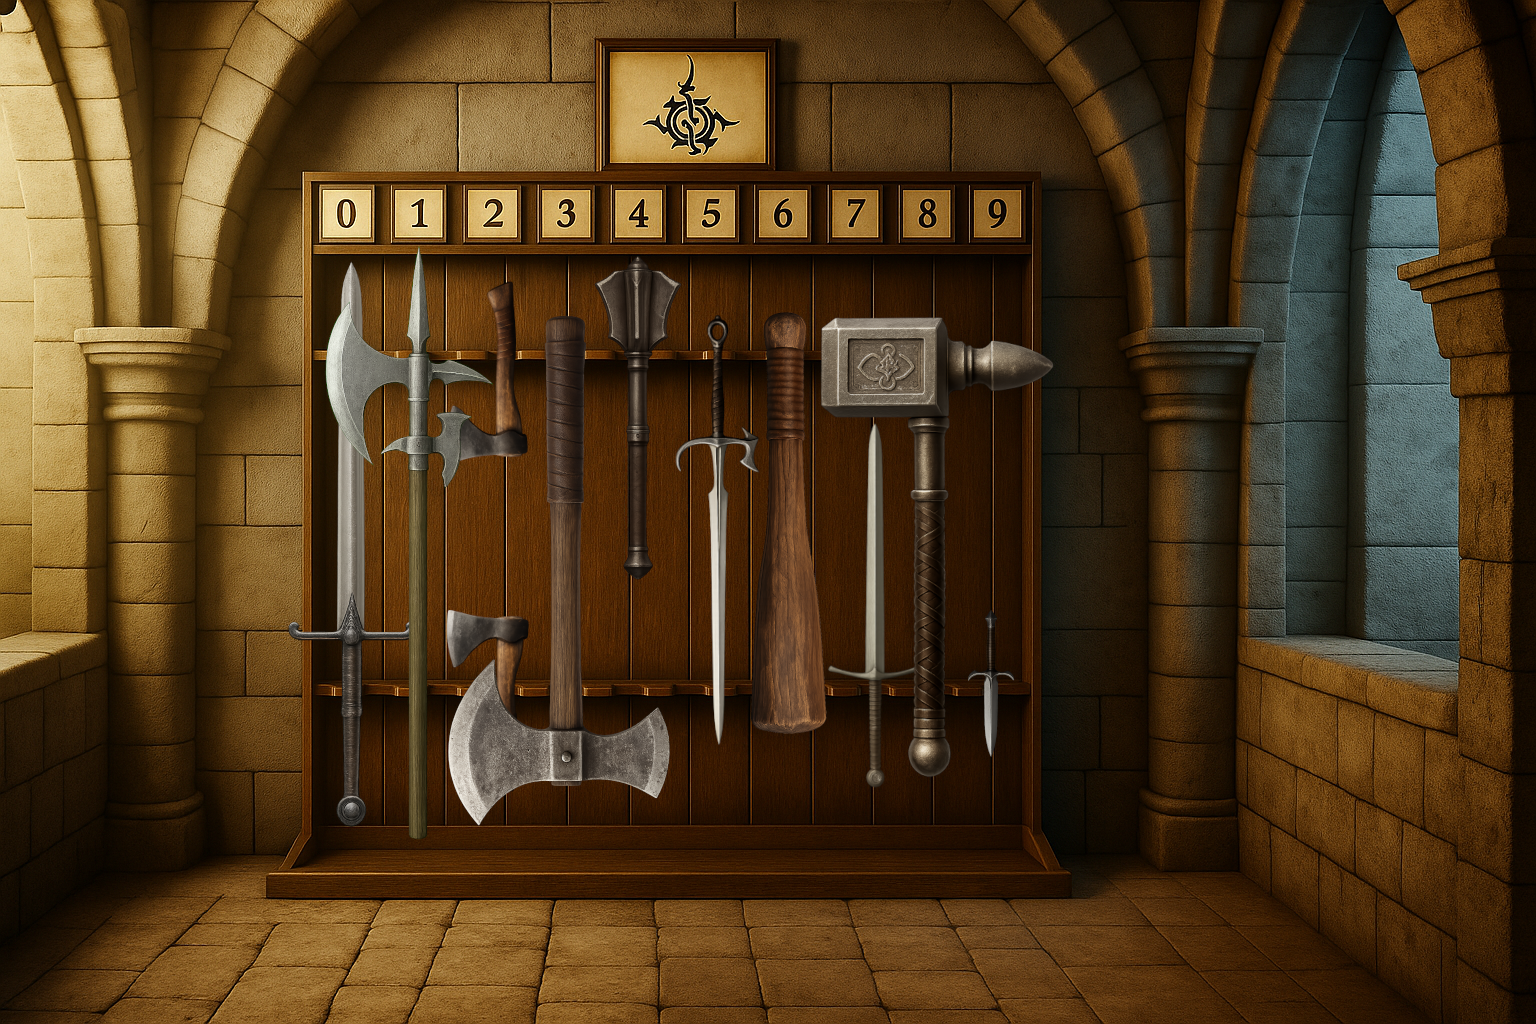
\includegraphics[width=\linewidth]{Puzzles/Weapon_Rack}

{\noindent\entryfont On this weapon rack, each number corresponds to a specific weapon: 4 is the mace, 9 is the dagger, and 7 is the longsword. To determine the proper order, players must arrange these three weapons by their damage dice - in ascending order from lowest to highest.}

\section*{Headmaster's Arcanum}\phantomsection\addcontentsline{toc}{section}{Headmaster's Arcanum}
{\entryfont The Arcanum is an impeccably maintained study, its polished marble floor reflecting the soft glow of arcane sconces. Every shelf and cupboard is completely void of books and artifacts, as though each volume was removed with deliberate care mere hours ago. There are no scuff marks or signs of disorder - only faint impressions on the dustless surfaces where tomes once rested. Drawers are closed flush, and the velvet rug lies perfectly centred before the fireplace. The sole remaining object is a leather-bound volume titled \textbf{"On the History of Master Arcanists"}, placed deliberately in the center of the mahogany desk. The lingering scent of fresh ink and parchment suggests Professor Ambric organized the space recently, then departed.}
\begingroup
	\DndSetThemeColor[PhbLightGreen]
	\begin{DndComment}{On the History of Master Arcanists}
		\textit{A book containing the history and description of the following spells:
		\begin{itemize}
			\item Jim's Magic Missile
			\item Melf's Acid Arrow
			\item Melf's Minute Meteor
			\item Leomund's Secret Chest
		\end{itemize}
		These spells can be copied into a spellbook.}
	\end{DndComment}
\endgroup